%%%%%%%%%%%%%%%%%%%%%%%%%%%%%%%%%%%%%%%%%%%%%%%%%%%%%%%%%%%%
%%  This Beamer template was created by Cameron Bracken.
%%  Anyone can freely use or modify it for any purpose
%%  without attribution.
%%
%%  Last Modified: January 9, 2009
%%

\documentclass[xcolor=x11names,compress]{beamer}

%% General document %%%%%%%%%%%%%%%%%%%%%%%%%%%%%%%%%%
\usepackage[utf8]{inputenc}
\usepackage[ngerman]{babel}
\usepackage{graphicx}
\usepackage{color}
\usepackage{tikz}
\usepackage{tabularx}
\usepackage[skins]{tcolorbox}
\usepackage{caption}
\usepackage{csquotes}
\usepackage{multicol,listings}
\usepackage{multirow}
\usepackage[absolute,overlay]{textpos}
\usepackage{transparent}
\usepackage{enumitem}
%%%%%%%%%%%%%%%%%%%%%%%%%%%%%%%%%%%%%%%%%%%%%%%%%%%%%%

%% Beamer Layout %%%%%%%%%%%%%%%%%%%%%%%%%%%%%%%%%%
\useoutertheme[subsection=false,infolines]{miniframes}
\useinnertheme{default}
\usefonttheme{serif}
\usepackage{palatino}

\setbeamertemplate{footline}[frame number]
%\setbeamertemplate{caption}[numbered]
\setbeamercolor{page number in head/foot}{fg=black}

\setbeamerfont{title like}{shape=\scshape}
\setbeamerfont{frametitle}{shape=\scshape}
\setbeamerfont{caption}{size=\tiny}
\setbeamerfont{caption name}{size=\tiny}

\setbeamercolor*{lower separation line head}{bg=DeepSkyBlue4} 
\setbeamercolor*{normal text}{fg=black,bg=white} 
\setbeamercolor*{alerted text}{fg=red} 
\setbeamercolor*{example text}{fg=black} 
\setbeamercolor*{structure}{fg=black} 
 
\setbeamercolor*{palette tertiary}{fg=black,bg=black!10} 
\setbeamercolor*{palette quaternary}{fg=black,bg=black!10} 

% Set right item bullet points in itemize (due to enumitem package)
\setitemize{label=\usebeamerfont*{itemize item}%
  \usebeamercolor[fg]{itemize item}
  \usebeamertemplate{itemize item}}

\renewcommand{\(}{\begin{columns}}
\renewcommand{\)}{\end{columns}}
\newcommand{\<}[1]{\begin{column}{#1}}
\renewcommand{\>}{\end{column}}

\beamertemplatenavigationsymbolsempty
\setcounter{tocdepth}{1}

\tcbset{enhanced}

% Set color for lstlisting
\definecolor{grey}{RGB}{105,105,105}

%%%%%%%%%%%%%%%%%%%%%%%%%%%%%%%%%%%%%%%%%%%%%%%%%%


\begin{document}

\begin{frame}
  \begin{figure}
    \begin{minipage}[c]{0.6\textwidth} 
    \tiny{Humboldt-Universität zu Berlin\\Mathematisch-Naturwissenschaftliche Fakultät\\Institut für Informatik\\Lehrstuhl Technische Informatik}
    \end{minipage}
    \hfill
    \begin{minipage}[c]{0.15\textwidth}
    \begin{figure}
      \includegraphics[width=\textwidth]{figures/HU_Logo}
    \end{figure}
    \end{minipage}
  \end{figure}

\title{\textbf{Measurements and Optimizations with Just-In-Time Code Generation on the OpenFlow Reference Implementation}}
\subtitle{KUVS-Prize, NetSys 2015 Cottbus}

\author{
  \vspace*{-1cm}
	\normalsize{\it Samuel Brack}\\
}
\date{March 11, 2015}
\titlepage
\end{frame}

%-----------------------------------------------------------------------------%

\section{\scshape Introduction}
\begin{frame}
  \centering\Huge{\insertsection}
\end{frame}

\subsection{\scshape Packet Classification}
\begin{frame}
  \frametitle{\insertsubsection}
  \begin{itemize}
    \item The Internet is growing constantly
    \item Data rates are in magnitudes of 100\ GBit/s
    \item Line speed packet classification is a necessity for powerful switches, routers and firewalls
    \item Budgets for network operation are low
  \end{itemize}
\end{frame}

\begin{frame}
  Packet Classification can be modeled as a function \textit{M}:
  \begin{tcolorbox}[colback=blue!5!white,colframe=blue!75!black,title=Definition,drop fuzzy shadow]
  \begin{tabularx}{\textwidth}{XX}
    Input&Packet \textit{P}, Rule set \textit{R}\\
    Output&Decision \textit{D}
  \end{tabularx}
  \end{tcolorbox}
  \begin{figure}
  \centering
  \includegraphics<1>[height=0.4\textheight]{figures/matching_function}
  \end{figure}
\end{frame}

%\subsection{\scshape OpenFlow}
%\begin{frame}
  %\frametitle{\insertsubsection}
  %OpenFlow ist eine Protokollspezifikation für Software Defined Networks:
  %\begin{itemize}
    %\item Zentrale Konfiguration von Netzwerkhardware.
    %\item Abstraktion der Aufgaben im Netzwerk von der eigentlichen Hardware.
    %\item Einfache Möglichkeit Netzwerke automatisch zu optimieren.
  %\end{itemize}
  %\pause
  %\begin{tcolorbox}[colback=blue!5!white,colframe=blue!75!black,title=Ziel dieser Arbeit,drop fuzzy shadow]
  %Verbesserung der Matching-Performance im Software-Switch der OpenFlow-Referenzimplementierung 1.0.
  %\end{tcolorbox}
%\end{frame}

\section{\scshape The Bitvector Algorithm}
\begin{frame}
  \centering\Huge{\insertsection}
\end{frame}

%\begin{frame}
  %Paketfilter sind häufig als einfache Liste von Regeln implementiert.
  %\begin{figure}
  %\centering
  %\includegraphics<1>[width=\textwidth]{figures/list_workflow-L1}
  %\includegraphics<2>[width=\textwidth]{figures/list_workflow-L1-2}
  %\includegraphics<3>[width=\textwidth]{figures/list_workflow-L1-3}
  %\includegraphics<4>[width=\textwidth]{figures/list_workflow-L1-4}
  %\end{figure}
%\end{frame}

\subsection{\scshape Basic Idea}
\begin{frame}
  \frametitle{\insertsubsection}
  $n:$ Number of rules
  \begin{tcolorbox}[colback=red!5!white,colframe=red!75!black,title=Problem,drop fuzzy shadow]
  Linear search (in a list) is slow, i.e. $\in \mathcal O(n)$.
  \end{tcolorbox}
  \pause
  \begin{tcolorbox}[colback=teal!5!white,colframe=teal!75!black,title=Idea,drop fuzzy shadow]
  Binary search possible in $\mathcal O(log\ n)$.\\
  \textit{Divide and conquer} over the relevant header fields.
  \end{tcolorbox}
  \pause
  \begin{tcolorbox}[colback=blue!5!white,colframe=blue!75!black,title=Possible solution,drop fuzzy shadow]
  The Bitvector algorithm.
  \end{tcolorbox}
\end{frame}

\begin{frame}
  Geometric representation of packet classification.
  \pause
  \begin{table}
  \centering
  \begin{tabularx}{0.7\textwidth}{c|X|X}
  Rule&Source&Destination\\
  \hline
  1&3 -- 11&4 -- 13\\
  2&1 -- 5&2 -- 5\\
  3&8 -- 13&0 -- 3\\
  \end{tabularx}
  \end{table}
  Nota bene:\\
  The first match \enquote{wins} and the search returns.
\end{frame}

\begin{frame}
  \begin{figure}
    \hspace*{-4cm}
    \includegraphics<1>[height=0.9\textheight]{figures/bitvector-L1}
    \includegraphics<2>[height=0.9\textheight]{figures/bitvector-L1_4}
    \includegraphics<3>[height=0.9\textheight]{figures/bitvector-L1_3_4}
    \includegraphics<4>[height=0.9\textheight]{figures/bitvector-L1-4}
    \includegraphics<5>[height=0.9\textheight]{figures/bitvector-L1-5}
    \includegraphics<6>[height=0.9\textheight]{figures/bitvector-L1-6}
    \includegraphics<7>[height=0.9\textheight]{figures/bitvector-L1-7}
    \includegraphics<8>[height=0.9\textheight]{figures/bitvector-L1-8}
    \includegraphics<9>[height=0.9\textheight]{figures/bitvector-L1-10}
  \end{figure}
  \begin{tikzpicture}[remember picture,overlay]  
    \node [xshift=-3.5cm,yshift=-2cm] at (current page.north east) {
      \begin{tabularx}{0.4\textwidth}{c|l|l}
        Rule&Source&Destination\\
        \hline
        \only<1>{\color{white}}1&
          \only<1>{\color{white}}3 -- 11&
          \only<1>{\color{white}}4 -- 13\\
        \only<1-2>{\color{white}}2&
          \only<1-2>{\color{white}}1 -- 5&
          \only<1-2>{\color{white}}2 -- 5\\
        \only<1-3>{\color{white}}3&
          \only<1-3>{\color{white}}8 -- 13&
          \only<1-3>{\color{white}}0 -- 3\\
      \end{tabularx}};
  \end{tikzpicture}
\end{frame}

\subsection{\scshape Lookup of Packets}
\begin{frame}
  \frametitle{\insertsubsection}
  Packets arrive and the matching rule is searched:
  \begin{table}
  \centering
  \begin{tabularx}{0.6\textwidth}{c|c|c}
  Packet&Source&Destination\\
  \hline
  P\ 1&4&4\\
  P\ 2&14&7\\
  \end{tabularx}
  \end{table}
\end{frame}

\begin{frame}
  \begin{figure}
  \hspace*{-4cm}
  \centering
  \includegraphics<1-2>[height=0.9\textheight]{figures/bitvector-L1-7_9_11_13_15}
  \includegraphics<3-4>[height=0.9\textheight]{figures/bitvector-L1-7_9_12_14_16}
  \end{figure}
  \begin{tikzpicture}[remember picture,overlay]  
    \node [xshift=-3.5cm,yshift=-2cm] at (current page.north east) {
      \begin{tabularx}{0.4\textwidth}{c|l|l}
        Packet&Source&Destination\\
        \hline
        P\ 1&4&4\\
        \only<1-2>{\color{white}}P\ 2&
          \only<1-2>{\color{white}}14&
          \only<1-2>{\color{white}}7\\
      \end{tabularx}};
  \end{tikzpicture}
  \begin{tikzpicture}[remember picture,overlay]  
    \node [xshift=-3.5cm,yshift=4cm] at (current page.south east) {
      \only<1-2>{\begin{tabularx}{0.15\textwidth}{ll}
        \only<1>{\color{white}}Source&\only<1>{\color{white}}1 1 0\\
        \only<1>{\color{white}}Destination&\only<1>{\color{white}}1 1 0\\
        \only<1>{\color{white}}\Large\&&\only<1>{\color{white}}\hrulefill\\
        \only<1>{\color{white}}Result&\only<1>{\color{white}}\only<2>{\color{red}}1 1 0\\
      \end{tabularx}}
      \only<3-4>{\begin{tabularx}{0.15\textwidth}{ll}
        \only<3>{\color{white}}Source&\only<3>{\color{white}}0 0 0\\
        \only<3>{\color{white}}Destination&\only<3>{\color{white}}1 0 0\\
        \only<3>{\color{white}}\Large\&&\only<3>{\color{white}}\hrulefill\\
        \only<3>{\color{white}}Result&\only<3>{\color{white}}\only<4>{\color{blue}}0 0 0\\
      \end{tabularx}}
      };
  \end{tikzpicture}
\end{frame}

%TODO
%\subsection{\scshape Runtime analysis}
%\begin{frame}
  %\frametitle{\insertsubsection}
  %$n:$  Number of rules, $k:$ Number of header fields,\\$w:$ Register width of the system in bit.
  %\pause
  %\begin{tcolorbox}[colback=red!5!white,colframe=red!75!black,title=Erinnerung: Lineare Suche,drop fuzzy shadow]
  %Die lineare Suche liegt in $\mathcal O(k \cdot n)$.
  %\end{tcolorbox}
  %\pause
  %\begin{tcolorbox}[colback=teal!5!white,colframe=teal!75!black,title=Bitvector-Algorithmus,drop fuzzy shadow]
  %\begin{itemize}[leftmargin=0cm]
    %\item[]<3-> Binäre Suche auf $k$ Headerfeldern,
    %\item[]<4-> bitweises ver-UND-en der $k$ Bitvektoren,
    %\item[]<5-> Suche nach dem ersten gesetzten Bit im Ergebnisvektor:
  %\end{itemize}
  %\centering
  %\begin{equation*}
  %\mathcal O(k \cdot log\ n \onslide<4->{+ \frac{n}{w} \cdot (k - 1)} \onslide<5->{ + n}).
  %\end{equation*}
  %\end{tcolorbox}
%\end{frame}
%EOT

\section{\scshape The JIT component}
\begin{frame}
  \centering\Huge{\insertsection}
\end{frame}

\subsection{\scshape Motivation}
\begin{frame}
  \frametitle{\insertsubsection}
  Assuming a static rule set, the binary search operates always in the same array.\\
  \begin{figure}
  \centering
  \includegraphics[height=5.5cm]{figures/matching_process}
  \end{figure}
\end{frame}

\begin{frame}
  \begin{tcolorbox}[colback=teal!5!white,colframe=teal!75!black,title=Reminder,drop fuzzy shadow]
  The matching function \textit{M} depends on the rule set \textit{R} and the packet \textit{P}.
  \end{tcolorbox}
  \begin{tcolorbox}[colback=red!5!white,colframe=red!75!black,title=Bottleneck,drop fuzzy shadow]
  The main bottleneck has been identified as the memory interface.
  \end{tcolorbox}
  \pause
  \begin{tcolorbox}[colback=blue!5!white,colframe=blue!75!black,title=Idea,drop fuzzy shadow]
  Further optimization by precomputing a function $M_R$.\\
  Implementation of a search tree per dimension in native code in order to \textbf{reduce memory accesses}.
  \end{tcolorbox}
  %\pause
  %\begin{tcolorbox}[colback=red!5!white,colframe=red!75!black,title=Nachteil,drop fuzzy shadow]
  %Bei jedem einzelnen Regel-Update erfolgt komplette Neuberechnung des Codes für den Suchbaum.
  %\end{tcolorbox}
\end{frame}

\begin{frame}
  \frametitle{\scshape Lookup steps}
  \begin{columns}[T] % align columns
    \begin{column}{.48\textwidth}
    \begin{tcolorbox}[colback=red!5!white,colframe=red!75!black,title=Standard bitvector,drop fuzzy shadow]
    \begin{enumerate}[label=\arabic*)]%TODO: schöner!
      \item \textit{k} binary search in all dimension.
      \item AND all result vectors.
      \item Search for first set bit.
    \end{enumerate}
    \end{tcolorbox}
    \end{column}
    \hfill
    \begin{column}{.48\textwidth}
    \begin{tcolorbox}[colback=blue!5!white,colframe=blue!75!black,title=Bitvector with JIT,drop fuzzy shadow]
    \begin{enumerate}[label=\arabic*)]%TODO: schöner!
      \item \textcolor{blue}{\textbf{\textit{k} calls of the JIT code.}}
      \item AND all result vectors.
      \item Search for first set bit.
    \end{enumerate}
    \end{tcolorbox}
    \end{column}
  \end{columns}
\end{frame}

\begin{frame}
  \begin{figure}
  \centering
  \includegraphics[scale=0.6]{figures/array_to_tree}
  \end{figure}
\end{frame}

%\subsection{\scshape JIT-Lookup}
%\begin{frame}
  %\frametitle{\insertsubsection}
  %\begin{figure}
  %\centering
  %\includegraphics<1>[height=0.7\textheight]{figures/match_in_tree-L1-2}
  %\includegraphics<2>[height=0.7\textheight]{figures/match_in_tree-L1_3}
  %\includegraphics<3>[height=0.7\textheight]{figures/match_in_tree-L1_4}
  %\includegraphics<4>[height=0.7\textheight]{figures/match_in_tree-L1_5}
  %\end{figure}
%\end{frame}

\section{\scshape Evaluation}
\begin{frame}
  \centering\Huge{\insertsection}
\end{frame}

%\subsection{\scshape Acceptance test}
%\begin{frame}
  %\frametitle{\insertsubsection}
  %Modular design of the OpenFlow switch allows testing the modules \enquote{against each other}.
  %\begin{figure}
  %\centering
  %\includegraphics<1>[height=6cm]{figures/acctest-L1}
  %\includegraphics<2>[height=6cm]{figures/acctest-L1-2}
  %\includegraphics<3>[height=6cm]{figures/acctest-L1-3}
  %\end{figure}
%\end{frame}

\subsection{\scshape Performance analysis}
\begin{frame}
  \frametitle{\insertsubsection}
  Evaluation of performance by a simple test setup in a virtual network using the \textsf{mininet} tool.
  \begin{itemize}
    \item Creation of random rule sets
    \item Derivation of packet streams from these rule sets using \textsf{classbench}.
    \item Inserting the rules into the switch.
    \item Sending the packets from the source.
    \item Counting the number of received packets on the receiver side.
  \end{itemize}
  \begin{figure}
  \centering
  \includegraphics[height=1cm]{figures/ofswitch-perftest}
  \end{figure}
\end{frame}

\begin{frame}
  Relative improvement compared to a linear list:
  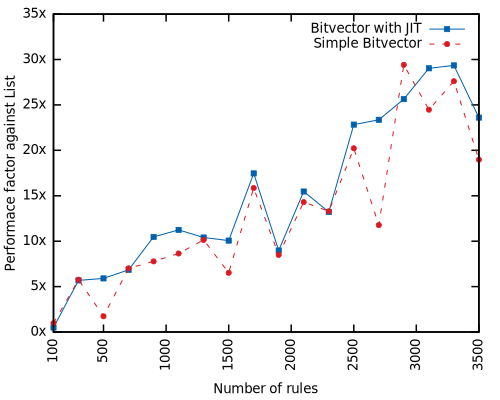
\includegraphics[height=0.9\textheight]{figures/eval_w_relative}
\end{frame}

\begin{frame}
  Time to update rule set:
  \includegraphics[height=0.9\textheight]{figures/eval_time}
\end{frame}

\begin{frame}
  Comparison of memory consumption:
  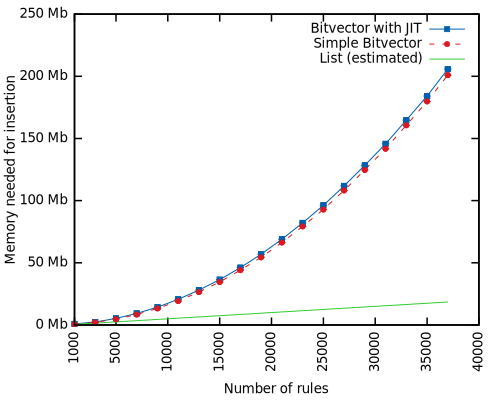
\includegraphics[height=0.9\textheight]{figures/eval_mem}
\end{frame}

\section{\scshape Conclusion}
\begin{frame}
  \centering\Huge{\insertsection}
\end{frame}

\subsection{\scshape Results}
\begin{frame}
  \begin{tcolorbox}[colback=teal!5!white,colframe=teal!75!black,title=Important Results,drop fuzzy shadow]
    \begin{itemize}
      \item Improving the performance of the switch by using the Bitvector algorithm.
      \item Implementation of a code generator for static rule sets.
      \item Evaluation and verification of the new components.
    \end{itemize}
  \end{tcolorbox}
  \pause
  \begin{tcolorbox}[colback=blue!5!white,colframe=blue!75!black,title=Future Work,drop fuzzy shadow]
    \begin{itemize}
      \item Incremental update of the JIT funktion when the rule set changes.
      \item Optimization of the JIT funktion using traffic patterns.
    \end{itemize}
  \end{tcolorbox}
\end{frame}

\section{}
\begin{frame}
  \frametitle{\scshape Questions?}
  \centering\Huge{?}
\end{frame}

\appendix
\section{\scshape Further Results}
\begin{frame}[noframenumbering]
  \frametitle{Aufteilung der Regelmenge}
  \centering\includegraphics[height=0.9\textheight]{figures/rule-thirds}
\end{frame}

\begin{frame}[noframenumbering]
  Ergebnisse für oberstes Drittel:
  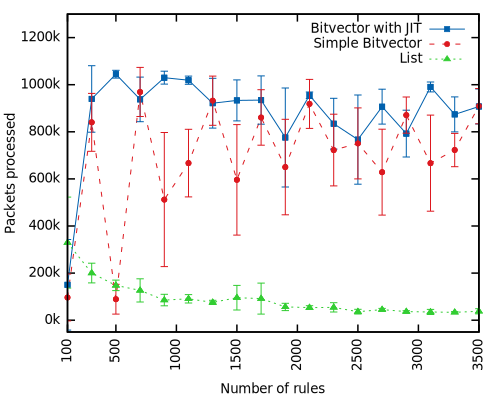
\includegraphics[height=0.9\textheight]{figures/eval_b}
\end{frame}

\begin{frame}[noframenumbering]
  Ergebnisse im mittleren Drittel:
  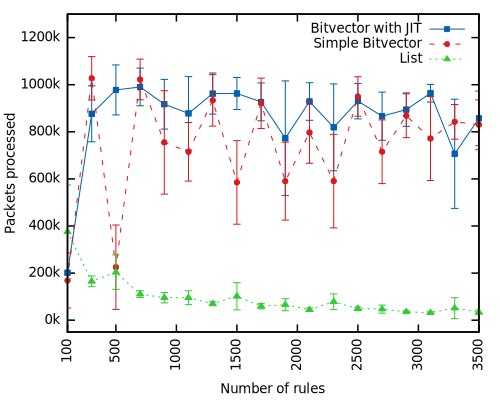
\includegraphics[height=0.9\textheight]{figures/eval_a}
\end{frame}

\begin{frame}[noframenumbering]
  Ergebnisse im letzten Drittel:
  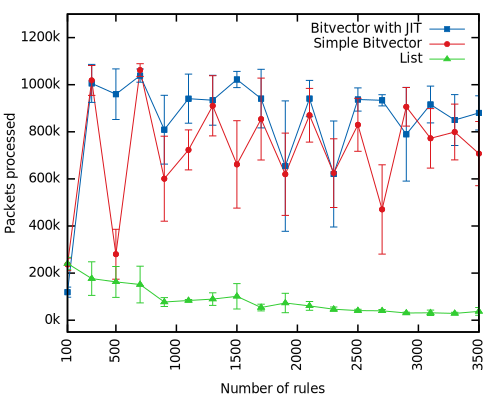
\includegraphics[height=0.9\textheight]{figures/eval_w}
\end{frame}

\begin{frame}[noframenumbering]
  Relative Verbesserung (oberstes Drittel):
  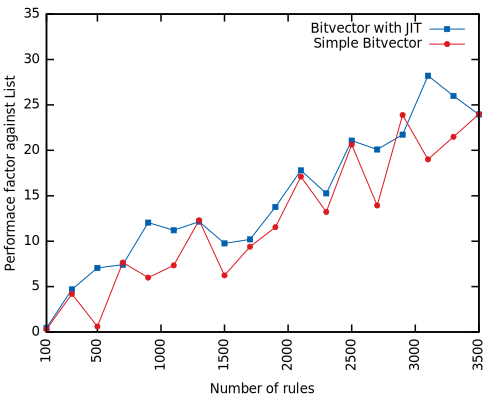
\includegraphics[height=0.9\textheight]{figures/eval_b_relative}
\end{frame}

\begin{frame}[noframenumbering]
  Relative Verbesserung (mittleres Drittel):
  \includegraphics[height=0.9\textheight]{figures/eval_a_relative}
\end{frame}

\begin{frame}[noframenumbering]
  Relative Verbesserung (letztes Drittel):
  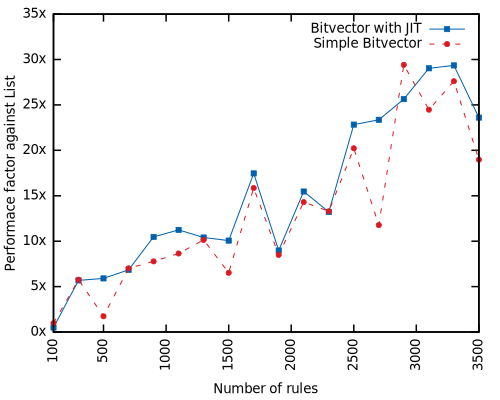
\includegraphics[height=0.9\textheight]{figures/eval_w_relative}
\end{frame}

\subsection{\scshape Generated Code}
\begin{frame}[noframenumbering]
  \only<2-7>{\begin{transparent}{0.4}}
  \only<-7>{\begin{multicols}{3}
  \lstinputlisting[
      language={[x86masm]Assembler},
      breaklines=true,
      numbers=left,
      texcl=true,
      xleftmargin=5.0ex,
      basicstyle=\tiny\ttfamily,
      keywordstyle=\bfseries\color{red},
      commentstyle=\itshape\color{grey},
      identifierstyle=\color{blue},
      morekeywords={retq,cmpq},
      numberstyle=\tiny
      ]
      {jit_listing.asm}
  \end{multicols}}
  
  \only<2-7>{\end{transparent}}

  \only<2>{\begin{textblock*}{64mm}(32mm,0.15\textheight)
    \begin{tcolorbox}[colback=red!5!white,colframe=red!75!black,title=Input into the function: 14,drop fuzzy shadow]
    \lstinputlisting[
      language={[x86masm]Assembler},
      breaklines=true,
      numbers=left,
      texcl=true,
      xleftmargin=5.0ex,
      basicstyle=\normalsize\ttfamily,
      keywordstyle=\bfseries\color{red},
      commentstyle=\itshape\color{grey},
      identifierstyle=\color{blue},
      morekeywords={retq,cmpq},
      numberstyle=\small,
      linerange={2-5},
      firstnumber=2
      ]
      {jit_listing.asm}
      \tcblower
      \centering{\includegraphics[height=0.35\textheight]{figures/match_in_tree-L1_9}}
    \end{tcolorbox}
  \end{textblock*}}
  
  \only<3>{\begin{textblock*}{64mm}(32mm,0.15\textheight)
    \begin{tcolorbox}[colback=red!5!white,colframe=red!75!black,title=Root node: compare with 5,drop fuzzy shadow]
    \lstinputlisting[
      language={[x86masm]Assembler},
      breaklines=true,
      numbers=left,
      texcl=true,
      xleftmargin=5.0ex,
      basicstyle=\normalsize\ttfamily,
      keywordstyle=\bfseries\color{red},
      commentstyle=\itshape\color{grey},
      identifierstyle=\color{blue},
      morekeywords={retq,cmpq},
      numberstyle=\small,
      linerange={7-10},
      firstnumber=7
      ]
      {jit_listing.asm}
      \tcblower
      \centering{\includegraphics[height=0.35\textheight]{figures/match_in_tree-L1_6_9}}
    \end{tcolorbox}
  \end{textblock*}}
  
  \only<4>{\begin{textblock*}{64mm}(32mm,0.15\textheight)
    \begin{tcolorbox}[colback=red!5!white,colframe=red!75!black,title=Root node: compare with 8,drop fuzzy shadow]
    \lstinputlisting[
      language={[x86masm]Assembler},
      breaklines=true,
      numbers=left,
      texcl=true,
      xleftmargin=5.0ex,
      basicstyle=\normalsize\ttfamily,
      keywordstyle=\bfseries\color{red},
      commentstyle=\itshape\color{grey},
      identifierstyle=\color{blue},
      morekeywords={retq,cmpq},
      numberstyle=\small,
      linerange={11-14},
      firstnumber=11
      ]
      {jit_listing.asm}
      \tcblower
      \centering{\includegraphics[height=0.35\textheight]{figures/match_in_tree-L1_6_9}}
    \end{tcolorbox}
  \end{textblock*}}
  
  \only<5>{\begin{textblock*}{64mm}(32mm,0.15\textheight)
    \begin{tcolorbox}[colback=red!5!white,colframe=red!75!black,title=Node C: compare with 11,drop fuzzy shadow]
    \lstinputlisting[
      language={[x86masm]Assembler},
      breaklines=true,
      numbers=left,
      texcl=true,
      xleftmargin=5.0ex,
      basicstyle=\normalsize\ttfamily,
      keywordstyle=\bfseries\color{red},
      commentstyle=\itshape\color{grey},
      identifierstyle=\color{blue},
      morekeywords={retq,cmpq},
      numberstyle=\small,
      linerange={46-49},
      firstnumber=46
      ]
      {jit_listing.asm}
      \tcblower
      \centering{\includegraphics[height=0.35\textheight]{figures/match_in_tree-L1_9_11}}
    \end{tcolorbox}
  \end{textblock*}}
  

  \only<6>{\begin{textblock*}{64mm}(32mm,0.15\textheight)
    \begin{tcolorbox}[colback=red!5!white,colframe=red!75!black,title=Node F: compare with 13,drop fuzzy shadow]
    \lstinputlisting[
      language={[x86masm]Assembler},
      breaklines=true,
      numbers=left,
      texcl=true,
      xleftmargin=5.0ex,
      basicstyle=\normalsize\ttfamily,
      keywordstyle=\bfseries\color{red},
      commentstyle=\itshape\color{grey},
      identifierstyle=\color{blue},
      morekeywords={retq,cmpq},
      numberstyle=\small,
      linerange={52-54},
      firstnumber=52
      ]
      {jit_listing.asm}
      \tcblower
      \centering{\includegraphics[height=0.35\textheight]{figures/match_in_tree-L1_9_10}}
    \end{tcolorbox}
  \end{textblock*}}
  
  \only<7>{\begin{textblock*}{64mm}(32mm,0.15\textheight)
    \begin{tcolorbox}[colback=red!5!white,colframe=red!75!black,title=Result: index 5,drop fuzzy shadow]
    \lstinputlisting[
      language={[x86masm]Assembler},
      breaklines=true,
      numbers=left,
      texcl=true,
      xleftmargin=5.0ex,
      basicstyle=\normalsize\ttfamily,
      keywordstyle=\bfseries\color{red},
      commentstyle=\itshape\color{grey},
      identifierstyle=\color{blue},
      morekeywords={retq,cmpq},
      numberstyle=\small,
      linerange={77-80},
      firstnumber=77
      ]
      {jit_listing.asm}
      \tcblower
      \centering{\includegraphics[height=0.35\textheight]{figures/match_in_tree-L1_8_9}}
    \end{tcolorbox}
  \end{textblock*}}
  
  \only<8>{
  \begin{multicols}{3}
  \lstinputlisting[
      language={[x86masm]Assembler},
      breaklines=true,
      numbers=left,
      texcl=true,
      xleftmargin=5.0ex,
      basicstyle=\tiny\ttfamily,
      keywordstyle=\bfseries\color{red},
      commentstyle=\itshape\color{grey},
      identifierstyle=\color{blue},
      morekeywords={retq,cmpq},
      numberstyle=\tiny
      ]
      {jit_listing.asm}
  \end{multicols}}
\end{frame}

\end{document}
